\documentclass[11pt]{article}

\usepackage[margin=1in]{geometry}
\usepackage{amsfonts}
\usepackage{amsmath}
\usepackage{graphicx}
\usepackage{algorithm}
\usepackage[noend]{algpseudocode}
\usepackage{url}
\usepackage{multirow}
\usepackage{authblk}
\usepackage{rotating}
\usepackage{xr}
\usepackage{natbib}

% \renewcommand{\thetable}{S\arabic{table}}   
% \renewcommand{\thefigure}{S\arabic{figure}}
% \renewcommand{\thealgorithm}{\arabic{algorithm}}

%\usepackage[style=nature,maxbibnames=5,mincitenames=1,maxcitenames=1]{biblatex}
% \renewbibmacro{in:}{%
%   \ifentrytype{article}{}{%
%   \printtext{\bibstring{in}\intitlepunct}}}
% \addbibresource{manuscript.bib}

\newcommand{\todo}[1]{}

\newcommand{\degree}{\ensuremath{^\circ}}

\renewcommand{\figurename}{Supplementary Figure}
\renewcommand{\tablename}{Supplementary Table}

\newfloat{suppalgorithm}{p}{cap}
\floatname{suppalgorithm}{Supplementary Algorithm}

\begin{document}

\title{Cloudbreak: Accurate and Scalable Genomic Structural Variation Detection in the Cloud with MapReduce \\
Supplementary Material}

\author[1,5]{Christopher W. Whelan \thanks{whelanch@ohsu.edu}}
\author[3,4]{Jeffrey Tyner}
\author[6]{Alberto L'Abbate}
\author[6]{Clelia Tiziana Storlazzi}
\author[4,5]{Lucia Carbone}
\author[1,2,5]{Kemal S\"onmez \thanks{sonmezk@ohsu.edu}}
\affil[1]{Institute on Development and Disability and Center for Spoken Language Understanding}
\affil[2]{Department of Medical Informatics \& Clinical Epidemiology}
\affil[3]{Program in Molecular and Cellular Biosciences}
\affil[4]{Behavioral Neuroscience Department}
\affil[5]{Oregon Health \& Science University, Portland, OR, USA}
\affil[6]{Department of Biology, University of Bari ``Aldo Moro'', Via G. Amendola 165/A, 70126, Bari, Italy}

\maketitle

\tableofcontents

\newpage

\section{Supplementary Figures} 

\begin{figure}[h]
\centering
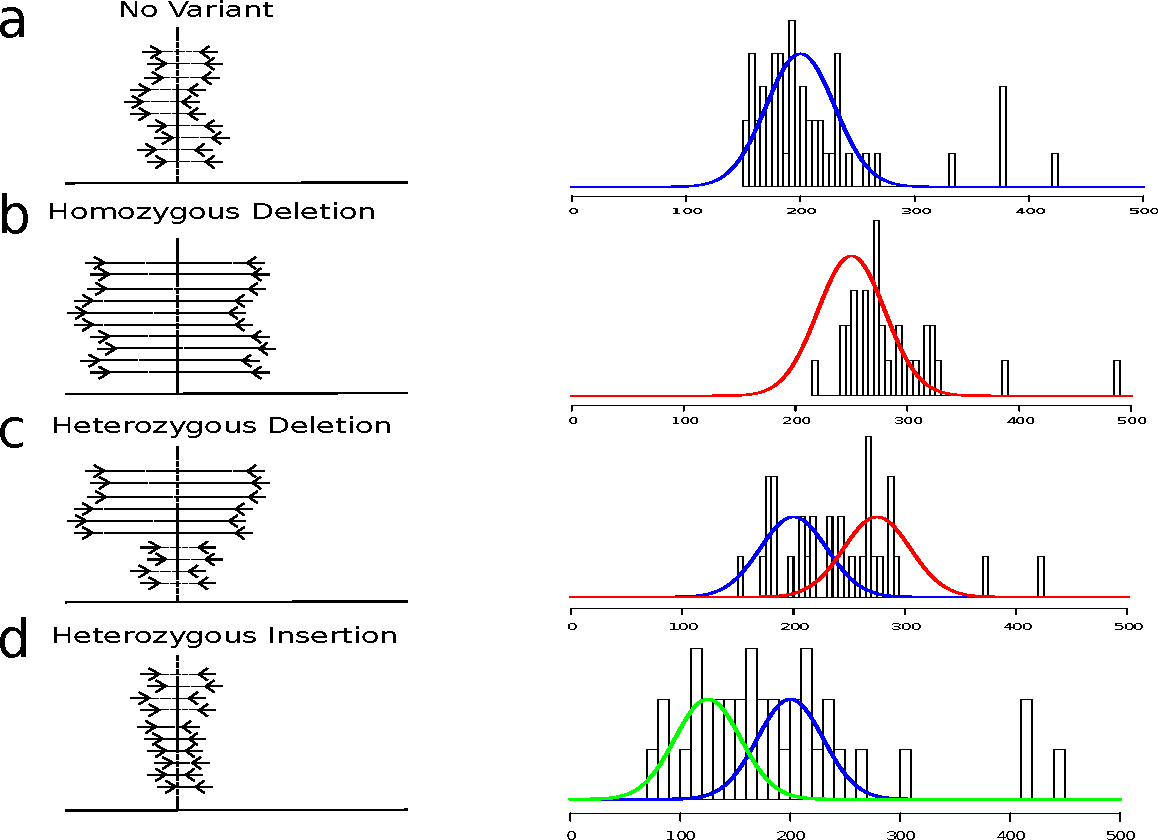
\includegraphics[width=1\textwidth]{insert_size_mixtures.pdf}
\caption{Illustration of insert size mixtures at individual genomic locations. A) There is no variant present at the location indicated by the vertical line (left), so the mix of insert sizes (right) follows the expected distribution of the library centered at 200bp, with a small amount of noise coming from low-quality mappings. B) A homozygous deletion of 50bp at the location has shifted the distribution of observed insert sizes. C) A heterozygous deletion at the location causes a mixture of normal and long insert sizes to be detected. D) A heterozygous small insertion shifts a portion of the mixture to have lower insert sizes.}
\label{insert_size_mixes}
\end{figure}

\clearpage

\begin{figure}[h]
\centering
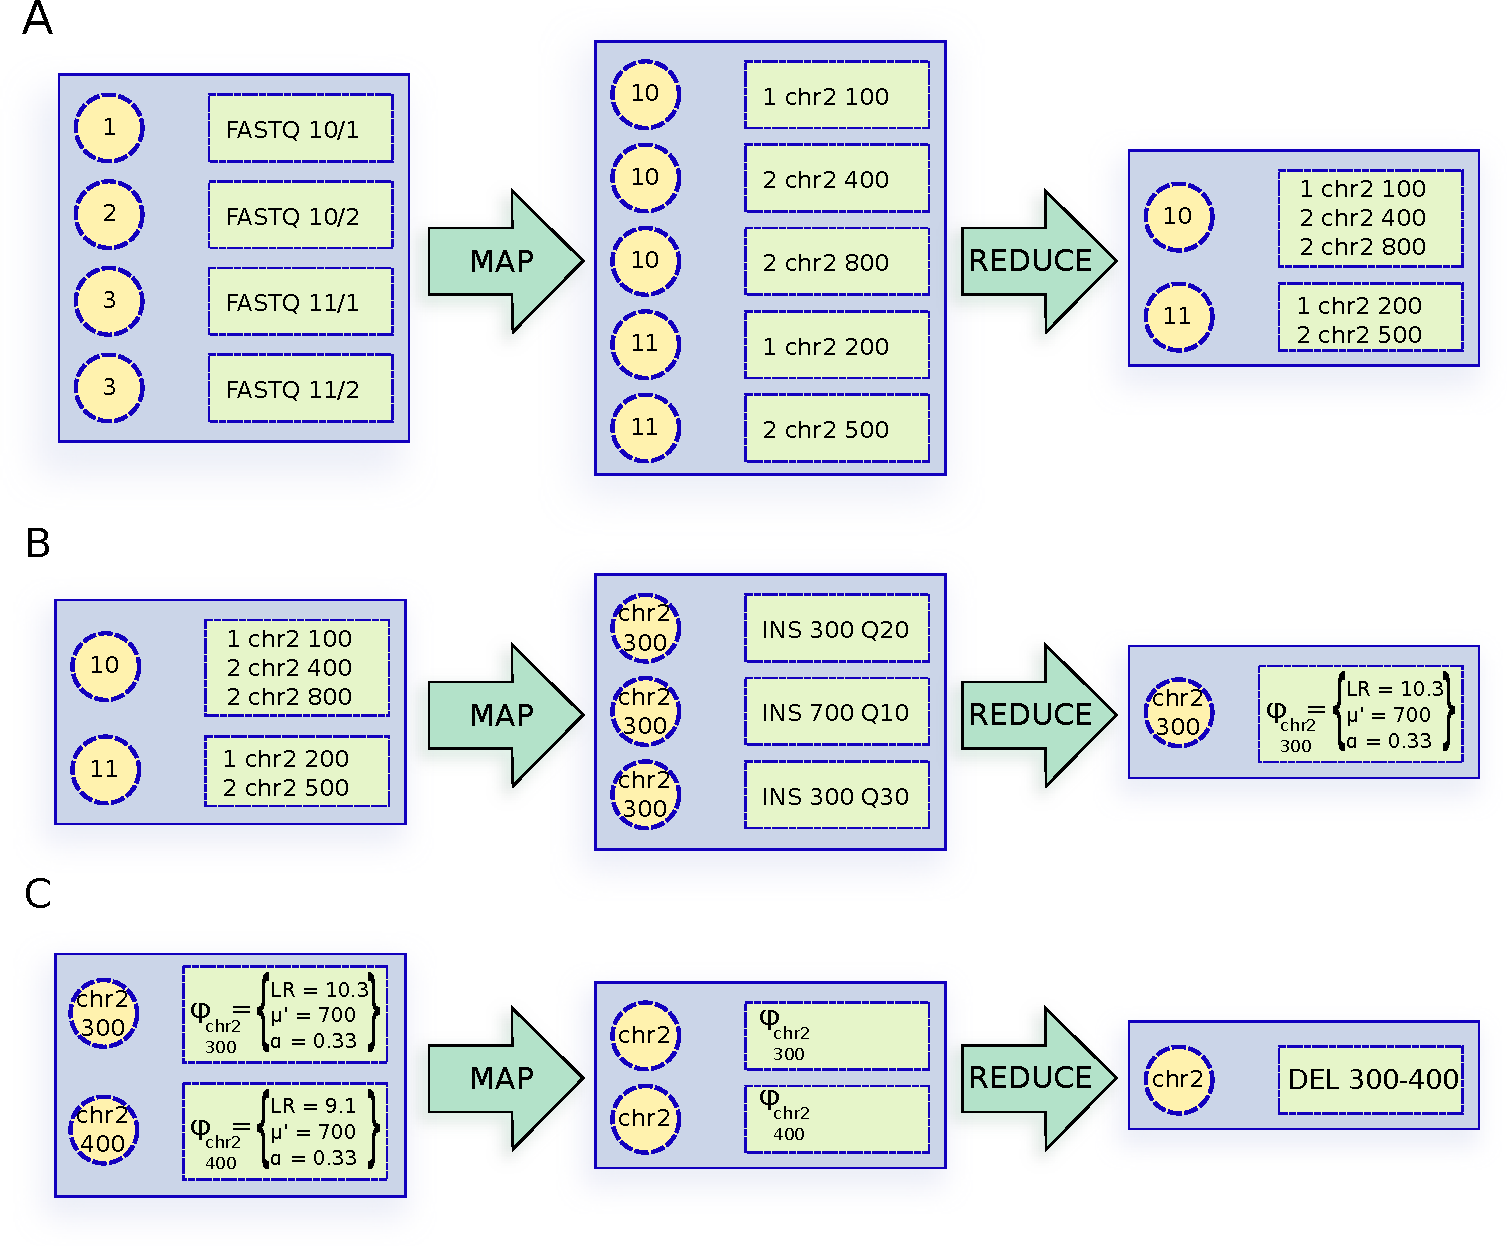
\includegraphics[width=1\textwidth]{cloudbreak_mapred_diagram.pdf}
\caption{An example of the Cloudbreak MapReduce algorithm. A) In the first MapReduce job, mappers scan input reads in FASTQ format and execute an alignment program in either paired-end or single-ended mode to generate read mappings. Reducers gather all alignments for both reads in each pair. B) In the second MapReduce job, mappers first emit information about each read pair (in this case the insert size and quality) under keys indicating the genomic location spanned by that pair. Only one genomic location is diagrammed here for simplicity. Reducers then compute features for each location on the genome by fitting a GMM to the distribution of spanning insert sizes. C) Mappers group all emitted features by their chromosome, and reducers find contiguous blocks of features that indicate the presence of a deletion.}
\label{algorithm_example}
\end{figure}

\clearpage

\begin{figure}
\centering
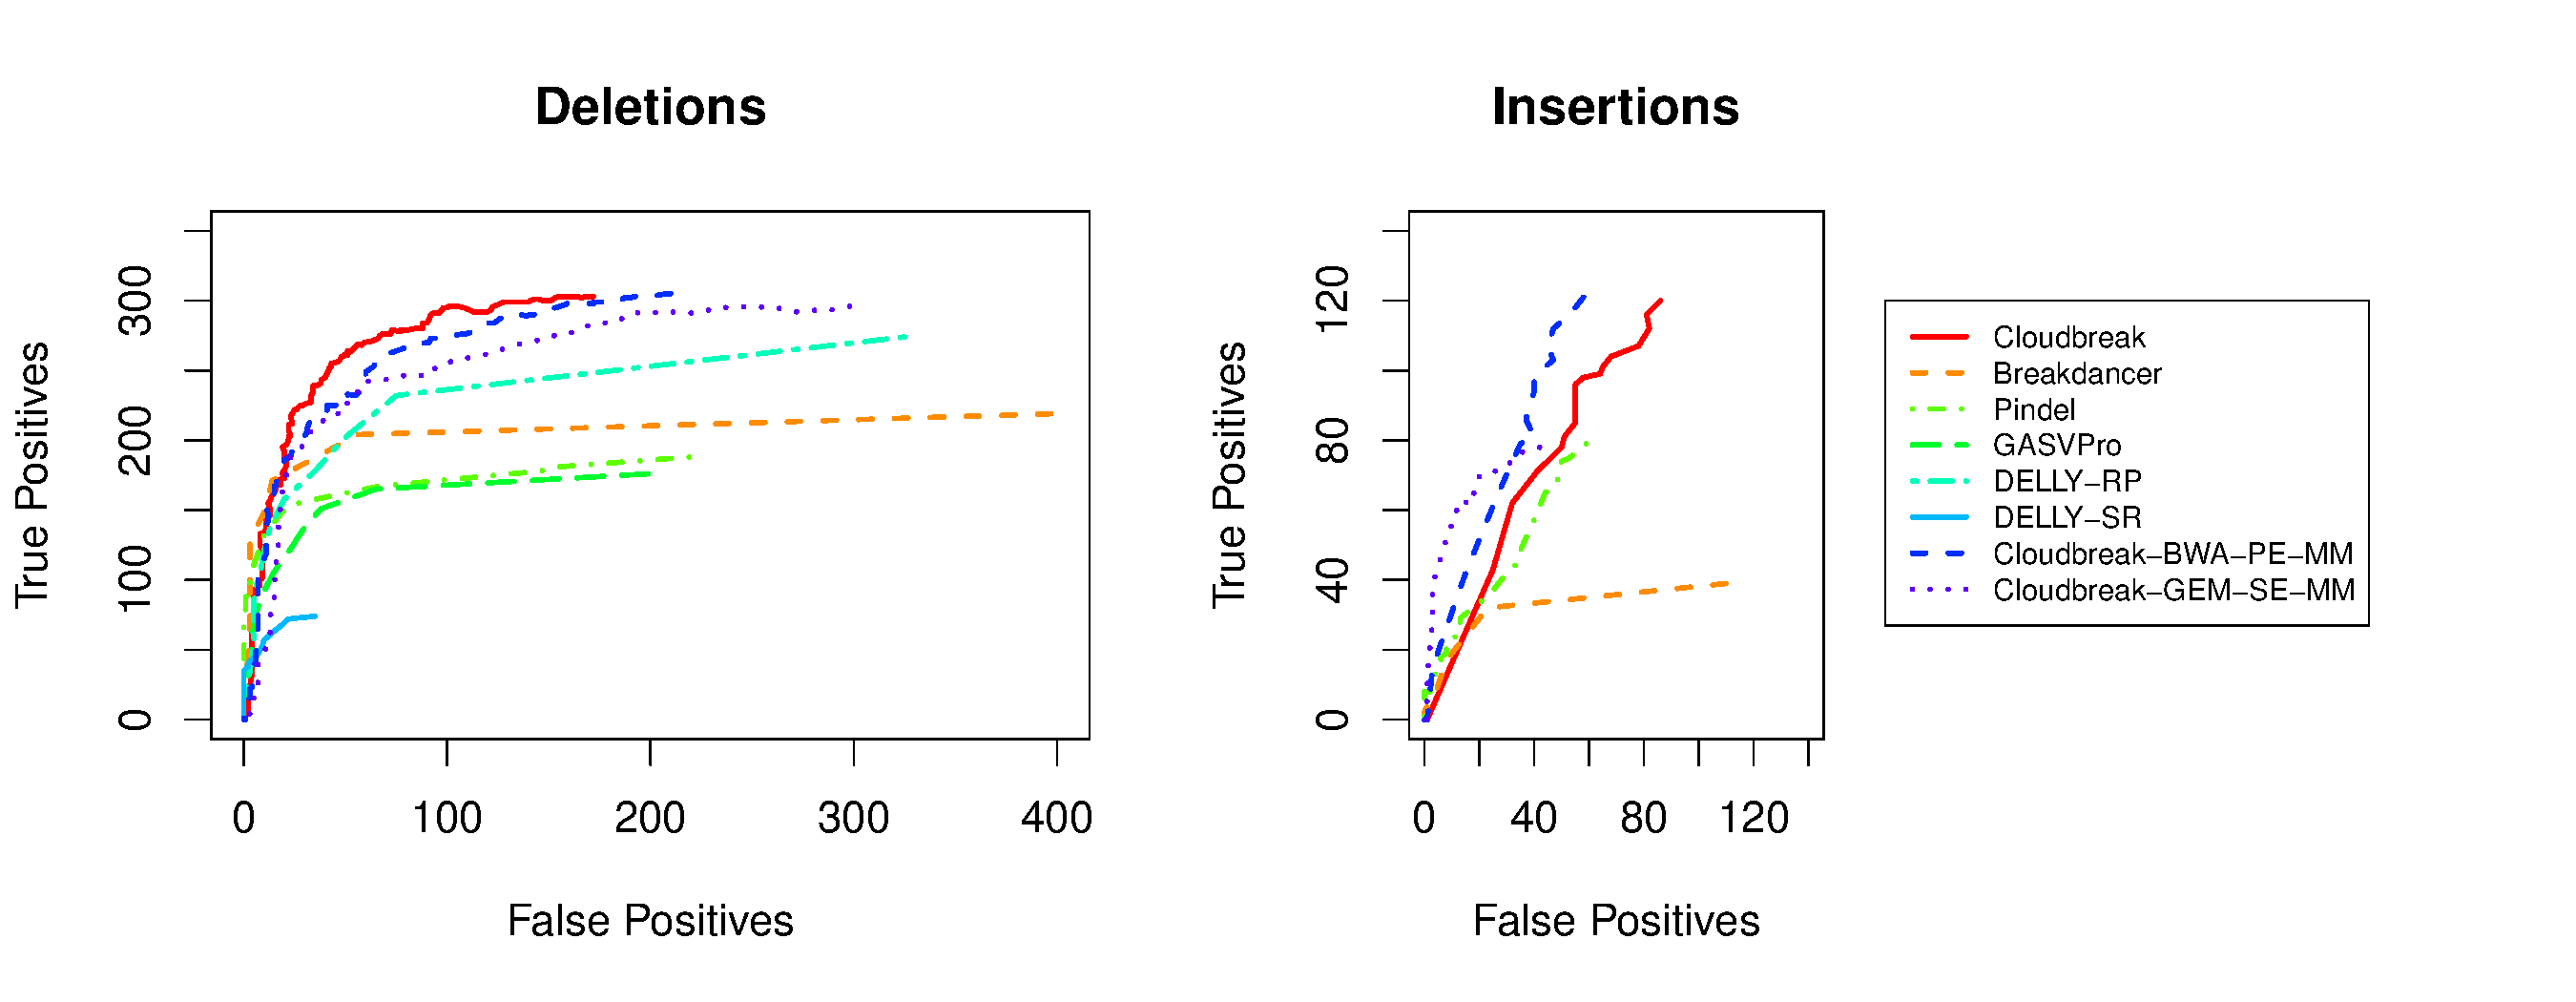
\includegraphics[width=1\textwidth]{CHR2SIM_ROCS_MULTIPLE_MAPPINGS.pdf}
\caption{Cloudbreak performance on the chromosome 2 simulation using different alignment strategies. ROC curves show the number of true positives and false positives for each operating point for deletions and insertions. The Cloudbreak alignment strategies are: 1) ``Cloudbreak'': Alignments generated with BWA in paired-end mode, reporting the best hit for each pair. 2) ``Cloudbreak-BWA-PE-MM'': Alignments generated with BWA in paired-end mode, reporting up to 25 additional hits for each mapping in SAM format using the \texttt{-n} and \texttt{-N} parameters for \texttt{bwa sampe} and the script \texttt{xa2multi.pl}. 3) ``Cloudbreak-GEM-SE-MM'': Alignments generated by running the GEM aligner in single-ended mode, reporting up to 1000 additional hits per alignment. GEM was executed in parallel using Hadoop tasks which wrap GEM version 1.362 (beta), with parameters \texttt{-e 6 -m 6 -s 2 -q ignore -d 1000 --max-big-indel-length 0},  requesting all hits for a read that are within an edit distance of 6 of the reference, within 2 strata of the best hit, with a maximum of 1000 possible alignments reported for each read. Considering multiple mappings improves Cloudbreak's specificity for insertions but decreases sensitivity to deletions.}
\label{alignment_comparison}
\end{figure}

\clearpage

\begin{figure}
\centering
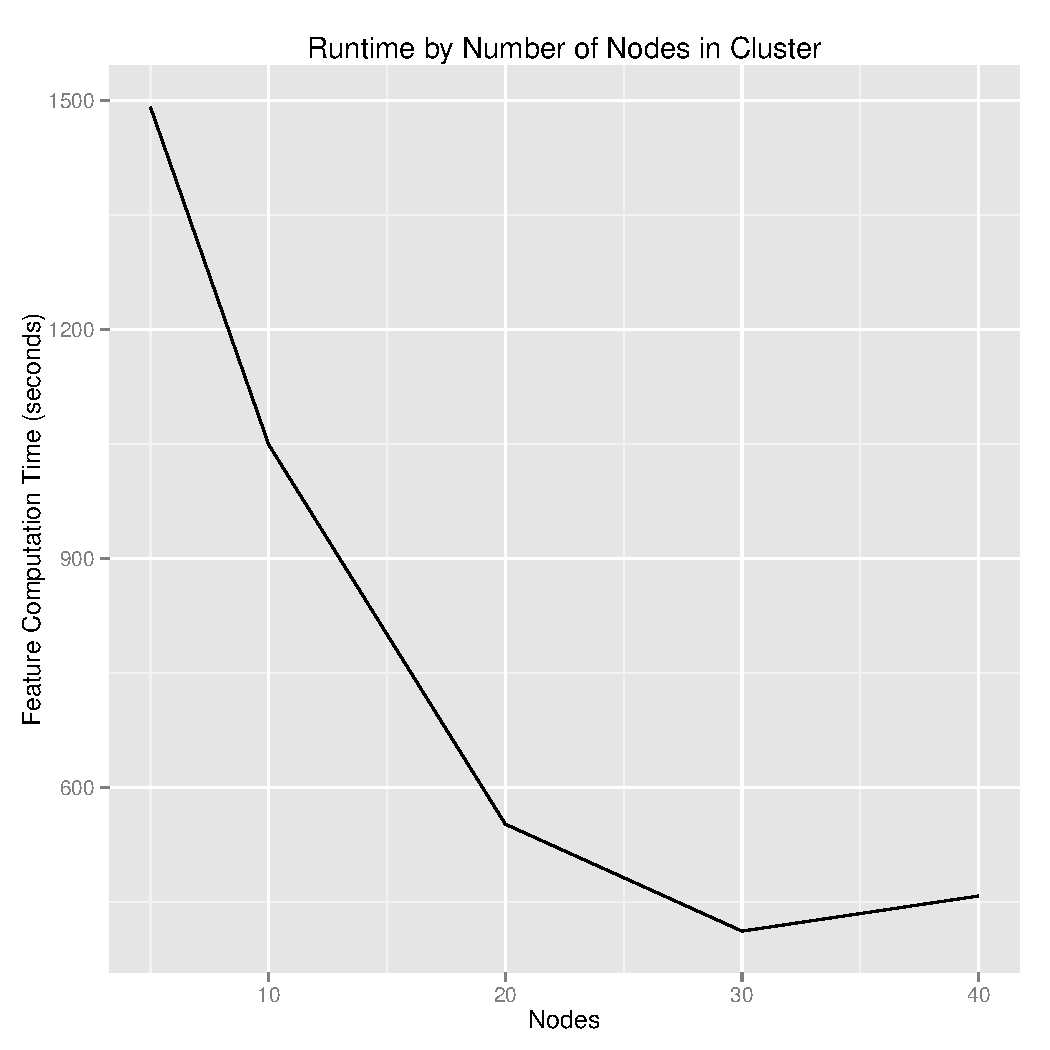
\includegraphics[width=1\textwidth]{runtimeByNodes.pdf}
\caption{Scalability of the Cloudbreak algorithm. Runtime of the Cloudbreak feature generation job for the simulated Chromosome 2 data is shown on Hadoop clusters consisting of varying numbers of compute nodes. Clusters were created in the Amazon Elastic Compute Cloud.}
\label{scalability}
\end{figure}

\clearpage

\begin{figure}
\centering
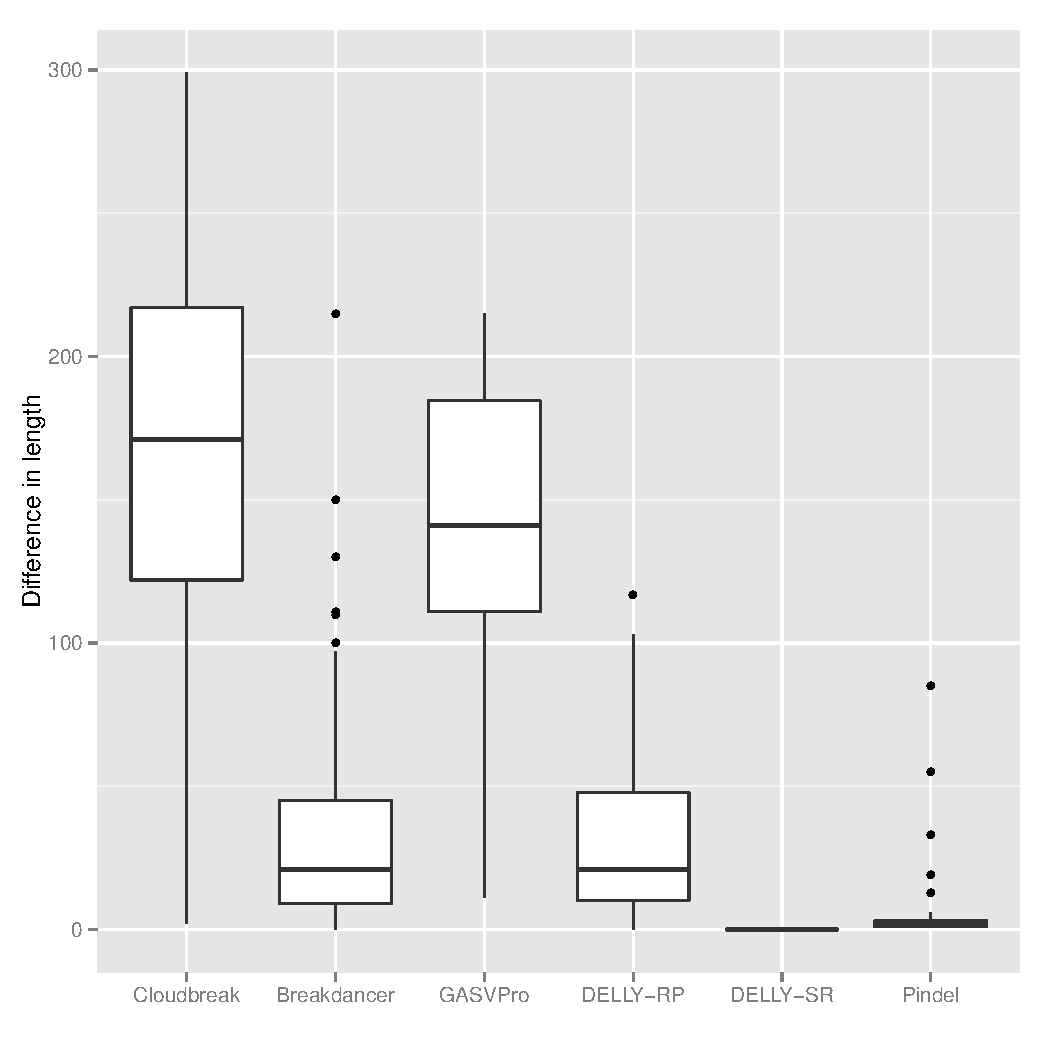
\includegraphics[width=1\textwidth]{breakpoint_resolution.pdf}
\caption{Breakpoint resolution for each tool for deletions on the Chromosome 2 simulated data. For each correctly predicted deletion, we calculated the difference in length between the true deletion and the prediction.}
\label{breakpoint_resolution}
\end{figure}

\clearpage

\begin{figure}
\centering
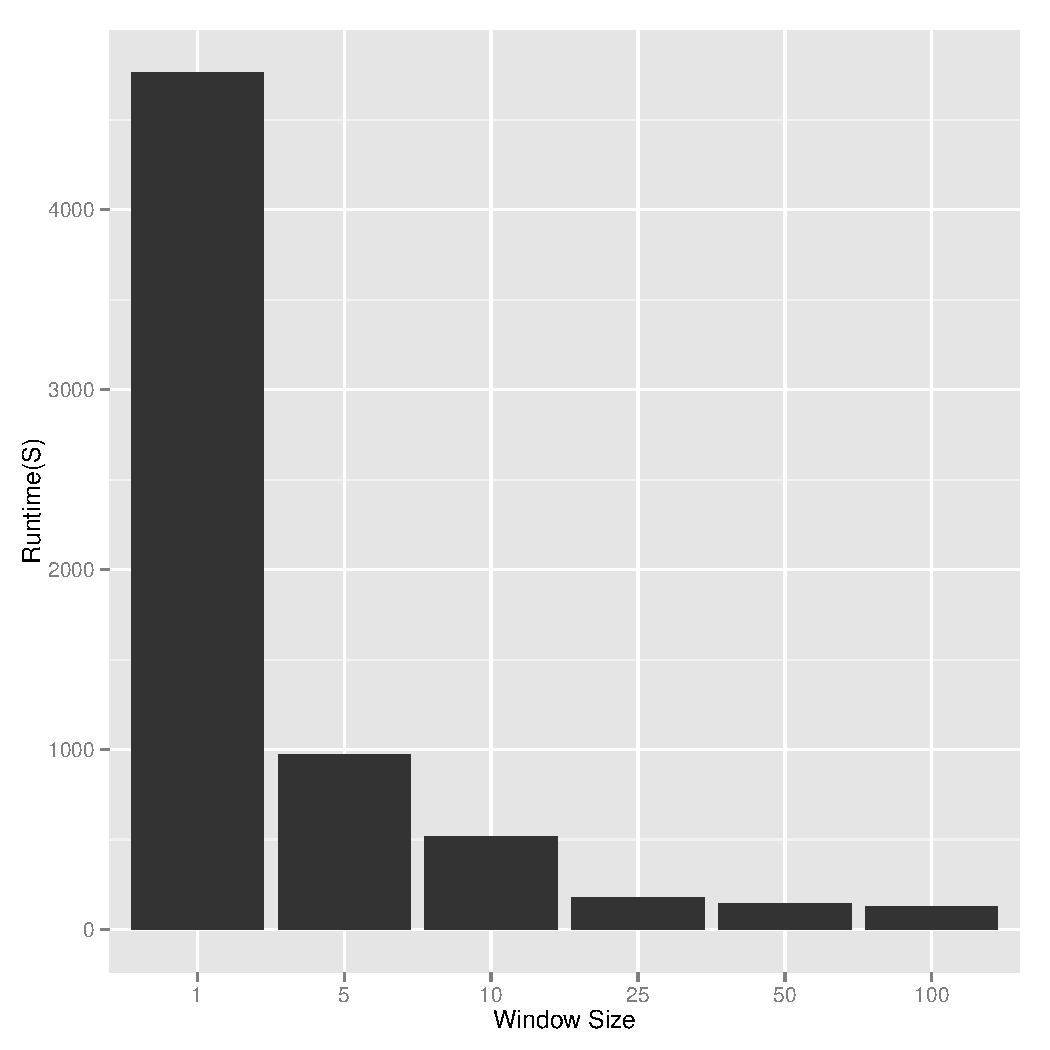
\includegraphics[width=.8\textwidth]{runtime_by_windowSize.pdf}
\caption[Cloudbreak runtimes with varying window sizes.]{Runtimes for Cloudbreak on the Chromosome 2 simulated data set using differing choices of window size. Runtimes include the feature computation and variant calling Cloudbreak Hadoop jobs.}
\label{figure_runtime_by_window_size}
\end{figure}

\begin{figure}
\centering
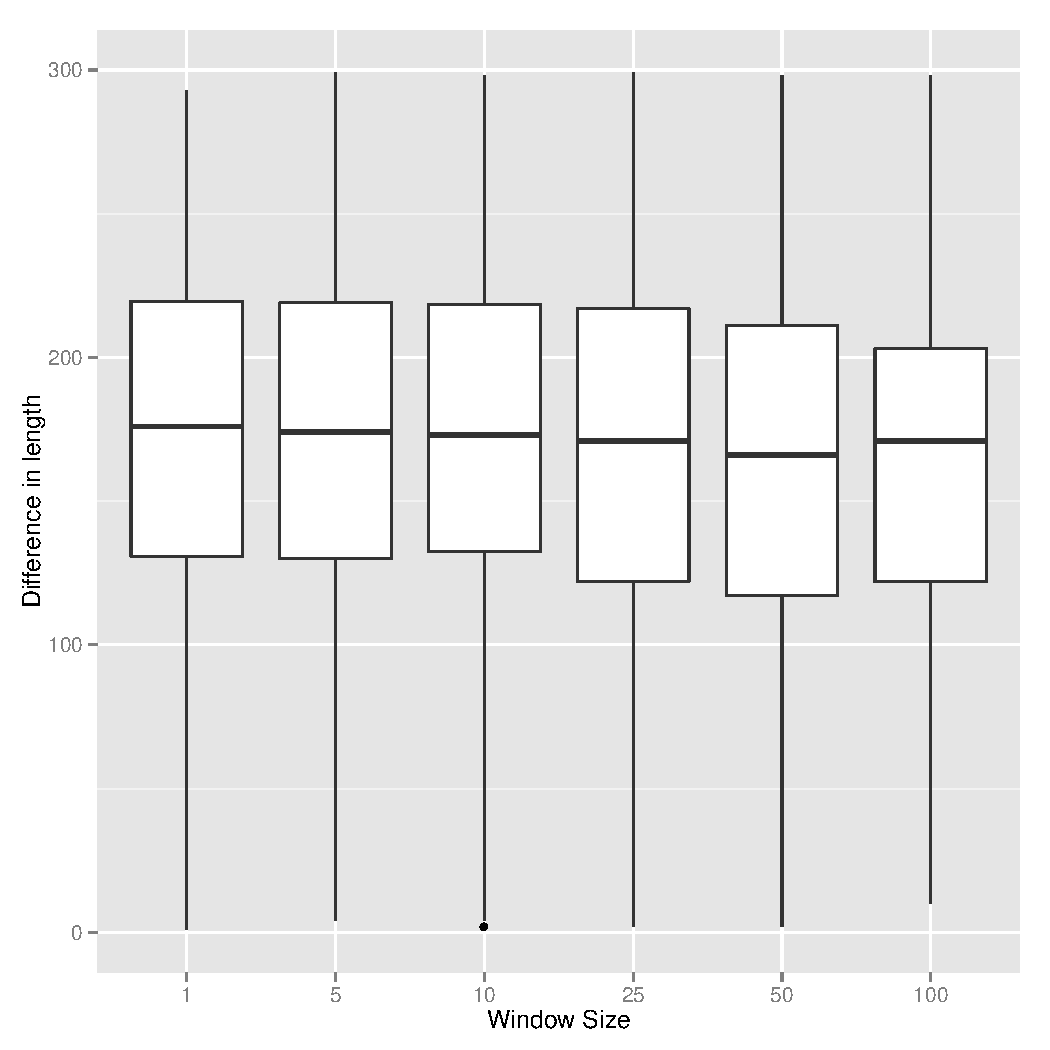
\includegraphics[width=.8\textwidth]{breakpoint_resolution_by_windowSize.pdf}
\caption[Cloudbreak breakpoint resolution with varying window sizes.]{Breakpoint resolution for Cloudbreak on the Chromosome 2 simulated data set using differing choices of window size.}
\label{breakpoint_resolution_by_windowSize}
\end{figure}

\clearpage

\section{Supplementary Tables}

\begin{table}[h]
\begin{center}
\begin{tabular}{r|r|rrr|rrr}
\multicolumn{2}{c}{}  & \multicolumn{3}{c}{Simulated Data} & \multicolumn{3}{c}{NA18507} \\
\hline
 & SV Types &  Single CPU & Parallel & Proc. &  Single CPU & Parallel & Proc.  \\ 
  \hline
  Cloudbreak & D,I &   NA    & 290 & 312    & NA         & 824 & 636 \\ 
  Breakdancer & D,I,V,T &  653   & NA       & NA          & 134,170 &  5,586 & 84 \\
  GASVPro & D,V   &  3,339  & NA       & NA         & 52,385  & NA & NA \\
  DELLY & D         &  1,964 & NA          & NA      & 30,311  & 20,224 & 84 \\
  Pindel & D,I,V,P         & 37,006 &  4,885     & 8          &  284,932  & 28,587 & 84 \\ 
  MoDIL & D,I        &  NA      & 52,547 & 250 & NA         & NA  & NA\\ 
   \hline
\end{tabular}
\end{center}
\caption{Runtimes (elapsed) on both data sets of each tool tested, in single-processor and parallel mode. For parallel runs, Proc. is the maximum number of simultaneously running processes or threads. All times are in seconds. The types of variants detected by each program are listed with the abbreviations: D - deletion; I - insertion; V - Inversion; P - duplication; T - translocation. Interchromosomal translocations are only detected by Breakdancer in single CPU mode. }
\label{runtimes}
\end{table}

\clearpage

\begin{table}[h]
\begin{center}
\begin{tabular}{rrrrrr}
  \hline
 & 40-100bp  & 101-250bp  & 251-500bp & 501-1000bp & $>$ 1000bp \\ 
 Total Number & 224 &  84 & 82 &  31 & 26\\ 
  \hline
  Cloudbreak  & \textbf{68} (17)  & \textbf{67} (\textbf{10}) &  \textbf{56} (\textbf{5}) & \textbf{11} (\textbf{3}) & \textbf{15} (\textbf{0}) \\ 
  Breakdancer & 52 (8)  & 49 (2) &  49 (0) & 7 (0) & 14 (\textbf{0}) \\ 
  GASVPro     & 35 (2)  & 26 (0) &  26 (0) & 2 (0) & 6 (\textbf{0}) \\ 
  DELLY-RP       & 22 (1)  & 56 (1) &  40 (0) & 8 (0) & 12 (\textbf{0}) \\ 
  DELLY-SR       & 0 (0)  & 2 (0) &  28 (0) & 2 (0) & 10 (\textbf{0}) \\ 
  Pindel      & 60 (\textbf{32})  & 16 (0) &  41 (2) & 1 (0) & 12 (\textbf{0})\\ 
   \hline
\end{tabular}
\end{center}
\caption{The number of simulated deletions in the 30X diploid chromosome 2 with Venter indels found by each tool at a 10\% FDR, as well as the number of those deletions that were discovered exclusively by each tool (in parentheses). The total number of deletions in each size class in the true set of deletions is shown in the second row of the header.}
\label{chr2DeletionPredsFDR10}
\end{table}

\newpage 

\begin{table}[h]
\begin{center}
\begin{tabular}{r|r|rr|rr|}
\multicolumn{2}{c}{}  & \multicolumn{4}{c}{Actual Genotypes} \\
\multicolumn{2}{c}{}  & \multicolumn{2}{c}{Simulated Data} & \multicolumn{2}{c}{NA18507} \\
\cline{3-6}
\multicolumn{2}{c|}{} &  Homozygous & Heterozygous & Homozygous & Heterozygous \\ 
\cline{2-6}
\multirow{2}{*}{\shortstack{Predicted \\ Genotypes}} & Homozygous & 35 & 2 &  96 & 21 \\
 & Heterozygous & 0 & 39 &  2 & 448 \\
\cline{2-6}
\end{tabular}
\end{center}
\caption{Confusion matrices for the predicted genotype of deletions found by Cloudbreak on both the simulated and NA18507 data sets.}
\label{deletionGenotypeaccuracy}
\end{table}

\newpage 

\begin{table}[h]
\begin{center}
\begin{tabular}{r|rrrrr}
 \hline
 Window Size & Calls & True Positives & Precision & Recall & F1 \\ 
 \hline
   1 & 274 & 228 & 0.832 & 0.57 & 0.677 \\ 
   5 & 268 & 228 & 0.851 & 0.57 & 0.683 \\ 
   10 & 258 & 223 & 0.864 & 0.557 & 0.678 \\ 
   25 & 240 & 217 & 0.904 & 0.542 & 0.678 \\ 
   50 & 215 & 194 & 0.902 & 0.485 & 0.631 \\ 
   100 & 162 & 141 & 0.87 & 0.352 & 0.502 \\  
\end{tabular}
\end{center}
\caption[Cloudbreak accuracy with varying window sizes.]{Accuracy measures for Cloudbreak on the Chromosome 2 simulated data set using different choices of window size. For each window size the same Cloudbreak score threshold was used (1.98).}
\label{chr2AccuracyByWindowSize}
\end{table}

\clearpage

\section{Supplementary Discussion}

\subsection{Fitting a GMM to the Observed Overlapping Insert Sizes}

We fit the parameters of the GMM using the Expectation-Maximization algorithm. Let $Y = y_{1,2, \ldots m}$ be the observed insert sizes at each location after filtering, and say the library has mean fragment size $\mu$ with standard deviation $\sigma$. We initialize the two components to have means $\mu$ and $\bar{Y}$, set the standard deviation of both components to $\sigma$, and set $\alpha = .5$. In the E step, we compute for each $y_i$ and GMM component $j$ the value $\gamma_{i,j}$, which is the normalized likelihood that $y_i$ was drawn from component $j$. We also compute $n_j = \sum_i{\gamma_{i,j}}$, the relative contributions of the data points to each of the two distributions. In the M step, we update $\alpha$ to be $n_2 - \left|Y\right|$, and set the mean of the second component to be $\frac{\sum_m{\gamma_{m,2}y_m}}{n_2}$. We treat the variance as fixed and do not update it, since under our assumptions the standard deviation of each component should always be $\sigma$. We repeat the E and M steps until convergence, or until a maximum number of steps has been taken.

\subsection{Filtering Incorrect and Ambiguous Mappings}

To handle incorrect and ambiguous mappings, we assume that in general they will not form normally distributed clusters in the same way that correct mappings will, and therefore use an outlier detection technique to filter the observed insert sizes for each location. We sort the observed insert sizes and define as an outlier an observation whose $k$th nearest neighbor, using differences between insert sizes as a measure of distance, is more than $n\sigma$ distant, where $k = 3$ and $n = 5$. The parameter $n=5$ represents the choice that only extreme outlier sets are to be eliminated and the parameter $k=3$ represents a trade-off in selecting size of the outlier set between eliminating true modes and allowing small outlier groups to skew the inference, which has been found by observing the distribution of outliers in data.

In addition, when the input data contains multiple possible mappings for each read pair, we calculate a score based on the probability that each mapping is correct relative to the other possible mappings. We then rank all observations at each genomic location, which in most cases include mappings from multiple read pairs, by their scores and use an \emph{adaptive quality cutoff} to filter observations: we discard all observations where the score is less than the maximum score observed at that location minus a constant $c$. This allows the use of more uncertain mappings in repetitive regions of the genome while restricting the use of low-quality mappings in unique regions. We compute mapping scores as follows: defining $\textsc{Mismatches}(a)$ to be the number of mismatches between a read and the reference genome in the alignment $a$, we compute the score $p^{k}_c$ of each end alignment by:

\[ p^{k}_c(a^{k}_{m,i}) = \frac{\exp({-\textsc{Mismatches}(a^{k}_{m,i})/2)}}{\sum_j{\exp(-\textsc{Mismatches}(a^{k}_{m,j})/2)}} \]

Where $k$ is the position of the read in the pair (i.e. 1,2), $m$ is the identifier of the read pair, and $i$ is the index of a particular possible mapping in the set of all possible mappings for that read. We then multiply $p_c(a^{1}_{m,i})$ and $p_c(a^{2}_{m,i})$ to give a score for that read pair. This score calculation was designed to give higher scores to the set of alignments with the smallest number of mismatches, while dividing smaller amounts of score among possible alignments with more mismatches than the best alignment in the set. When the data only contains one possible mapping for each read pair, as is the case in the experiments reported in the main manuscript, all read pairs receive a score of 1 under this scheme and therefore the adaptive quality cutoff is not invoked.

\subsection{Simulated and Biological Data Sets}\label{section_eval_data_sets}

As has been observed elsewhere, there is no available test set of real Illumina sequencing data from a sample that has a complete annotation of SVs from the reference. Therefore, testing with simulated data is important to fully characterize an algorithm's performance characteristics. On the other hand, it is important that the simulated data contain realistic SVs that follow patterns of SVs observed in real data. To address this, we took one of the most complete lists of SVs from a single sample available, the list of homozygous insertions and deletions from the genome of J. Craig Venter~\citep{Levy:2007fb}. Using these variants, we simulated a 30X read coverage data set for a diploid human Chromosome 2 with a mix of homozygous and heterozygous variants.  Since there are relatively few heterozygous insertions and deletions annotated in the Venter genome, we used the set of homozygous indels contained in the HuRef data (\texttt{HuRef.homozygous\_indels.061109.gff}) and randomly assigned each variant to be either homozygous or heterozygous with uniform probability. Based on this genotype, we applied each variant to one or both of two copies of the human GRCh36 chromosome 2 reference sequence. We then simulated paired Illumina reads from these modified references using \emph{dwgsim} from the DNAA software package (\url{http://sourceforge.net/apps/mediawiki/dnaa/}). We simulated 100bp reads with a mean fragment size of 300bp and a standard deviation of 30bp, and generated 15X coverage for each modified sequence. Pooling the reads from both simulations gives 30X coverage for a diploid sample with a mix of homozygous and heterozygous insertions and deletions.

We downloaded a data set of reads taken from a DNA sample of Yoruban individual NA18507, experiment ERX009609 from the Sequence Read Archive. This sample was sequenced on the Illumina Genome Analyzer II platform with 100bp paired end reads and a mean fragment size (minus adapters) of 300bp, with a standard deviation of 15bp, to a depth of approximately 37X coverage.

To create a gold standard set of insertions and deletions to test against, we pooled annotated variants discovered by three previous studies on the same sample. These included data from the Human Genome Structural Variation Project reported by Kidd et al.~\citep{Kidd:2008p926}, a survey of small indels conducted by Mills et al.~\citep{Mills:2011fi}, and insertions and deletions from the merged call set of the Phase 1 release of the 1000 Genomes Project~\citep{GenomesProjectConsortium:2012co} which were genotyped as present in NA18507. We merged any overlapping calls of the same type into the region spanned by their unions. It should be noted that the 1000 Genomes call set was partially produced using DELLY and BreakDancer, and therefore those calls are ones that those tools are sensitive to, biasing this test in their favor.

\subsection{Parameters Used for Alignment and SV Detection}

We aligned simulated reads to hg18 chromosome 2, NA18507 reads to the hg19 assembly. Alignments for all programs, unless otherwise noted, were found using BWA \texttt{aln} version 0.6.2-r126, with parameter \texttt{-e 5} to allow for longer gaps in alignments due to the number of small indels near the ends of larger indels in the Venter data set. We also tested the effect of including multiple possible mapping locations for ambiguously mapped reads in results reported in Supplementary Figure~\ref{alignment_comparison}. For those tests, we used two different sets of reads with multiple mapping locations reported. The first used alignments generated with BWA in paired-end mode, reporting up to 25 additional hits for each mapping  using the \texttt{-n} and \texttt{-N} parameters for \texttt{bwa sampe} and the script \texttt{xa2multi.pl}. For the second, we attempted to generate an exhaustive list of possible mapping locations by running the GEM aligner in single-ended mode on each read in each pair individually, reporting up to 1000 additional hits per alignment. GEM was executed in parallel using Hadoop tasks which wrap GEM version 1.362 (beta), with parameters \texttt{-e 6 -m 6 -s 2 -q ignore -d 1000 --max-big-indel-length 0}. These parameters request all hits for a read that are within an edit distance of 6 of the reference, within 2 strata of the best hit, with a maximum of 1000 possible alignments reported for each read. GASVPro also accepts ambiguous mappings but expects them to be realigned with a more sensitive alignment tool; following the details given in their manuscript we extracted read pairs that did not align concordantly with BWA and re-aligned them with Novoalign V2.08.01, with parameters \texttt{-a -r -Ex 1100 -t 250}. 

We ran Cloudbreak with a median filter window size of 5 genomic windows, an adaptive quality cutoff of 6, and a minimum coverage after filtering at each window of 3 spanning read pairs (parameters \texttt{--maxLogMapqDiff 6 --minCleanCoverage 3} on the feature generation step and \texttt{--medianFilterWindow 5} on the variant extraction steps). We chose these parameters based on limited tuning on the simulated data set.

We ran BreakDancer version 1.1\_2011\_02\_21 in single threaded mode by first executing \texttt{bam2cfg.pl} and then running \texttt{breakdancer\_max} with the default parameter values.  To run BreakDancer in parallel mode we first ran \texttt{bam2cfg.pl} and then launched parallel instances of \texttt{breakdancer\_max} for each chromosome using the \texttt{-o} parameter. We ran DELLY version 0.0.9 with the \texttt{-p} parameter and default values for other parameters. For the parallel run of DELLY we first split the original BAM file with BamTools \citep{Barnett:2011hm}, and then ran instances of DELLY in parallel for each BAM file. We ran GASVPro version 1.2 using the \texttt{GASVPro.sh} script and default parameters. Pindel 0.2.4t was executed with default parameters in single CPU mode, and executed in parallel mode for each chromosome using the \texttt{-c} option. We executed MoDIL with default parameters except for a \texttt{MAX\_DEL\_SIZE} of 25000, and processed it in parallel on our cluster with a step size of 121475. To execute other SV detection tools in parallel we wrote simple scripts to submit jobs to the cluster using the HTCondor scheduling engine \citep{condor-practice} with directed acyclic graphs to describe dependencies between jobs. 

\subsection{SV Prediction Evaluation}

We use the following criteria to define a true prediction given a gold standard set of deletion and insertion variants to test against: A predicted deletion is counted as a true positive if a) it overlaps with a deletion from the gold standard set, b) the length of the predicted call is within 300bp (the library fragment size in both our real and simulated libraries) of the length of the true deletion, and c) the true deletion has not already been discovered by another prediction from the same method. For evaluating insertions, each algorithm produces insertion predictions that define an interval in which the insertion is predicted to have occurred with start and end coordinates $s$ and $e$ as well as the predicted length of the insertion, $l$. The true insertions are defined in terms of their actual insertion coordinate $i$ and their actual length $l_a$. Given this information, we modify the overlap criteria in a) to include overlaps of the intervals $\langle s,\max{\left(e,s+l\right)} \rangle$ and $\langle i,i+l_a \rangle$. In this study we are interested in detecting events larger than 40bp, because with longer reads, smaller events can be more easily discovered by examining gaps in individual reads. Both Pindel and MoDIL make many calls with a predicted event size of under 40bp, so we remove those calls from the output sets of those programs. Finally, we exclude from consideration calls from all approaches that match a true deletion of less than 40bp where the predicted variant length is less than or equal to 75bp in length.

\subsection{Runtime Analysis}

We implemented and executed Cloudbreak on a 56-node Hadoop cluster, with 636 map slots and 477 reduce slots. Not including alignment time, we were able to process the Chromosome 2 simulated data in under five minutes, and the the NA18507 data set in under 15 minutes. For the simulated data set we used 100 reducers for the compute SV features job; for the real data set we used 300. The bulk of Cloudbreak's execution is spent in the feature generation step. Extracting deletion and insertion calls take under two minutes each for both the real and simulated data sets; the times are equal because each reducer is responsible for processing a single chromosome, and so the runtime is bounded by the length of time it takes to process the largest chromosome. 

In Supplementary Table \ref{runtimes} we display a comparison of runtimes on the real and simulated data sets for all of the tools evaluated in this work. Each tool varies in the amount of parallelization supported. We report runtimes for tools run in their default single-threaded mode, as well as for levels of parallelization achievable with basic scripting, noting that one of the key advantages of Hadoop/MapReduce is the ability to scale parallel execution to the size of the available compute cluster without any custom programming. To execute the tools in parallel mode we wrote simple scripts to submit jobs to the cluster using the HTCondor scheduling engine (\url{http://research.cs.wisc.edu/htcondor/}) with directed acyclic graphs to describe dependencies between jobs.  Pindel allows multi-threaded operation on multicore servers. Pindel and Breakdancer allow processing of a single chromosome in one process, so it is possible to execute all chromosomes in parallel on a cluster that has a job scheduler and shared filesystem. Breakdancer has an additional preprocessing step (\texttt{bam2cfg.pl}) which runs in a single thread. DELLY suggests splitting the input BAM file by chromosome, after which a separate DELLY process can be executed on the data for each chromosome; splitting a large BAM file is a time consuming process and consumes most of the time in this parallel workflow, in fact making it faster to run in single-threaded mode. GASVPro allows parallelization of the MCMC component for resolving ambiguously mapped read pairs; however, this requires a significant amount of custom scripting, and we did not find that the MCMC module consumed most of the runtime in our experiments, so we do not attempt to parallelize this component. The MoDIL distribution contains a set of scripts that can be used to submit parallel jobs to the SGE scheduling engine or modified for other schedulers; we adapted these for use in our cluster.

In parallel execution, the total time to execute is bounded by the runtime of the longest-running process. In the case of chromosome-parallelizable tools including Breakdancer, Pindel, and DELLY, this is typically the process working on the largest chromosome.\footnote{We note that one Breakdancer process, handling an unplaced contig in the hg19 reference genome, never completed in our runs and had to be killed manually; we exclude that process from our results.} In the case of MoDIL's run on the simulated data, we found that the different processes varied widely in their execution times, likely caused by regions of high coverage or with many ambiguously mapped reads. Cloudbreak mitigates this problem during the time-consuming feature generation process by using Hadoop partitioners to randomly assign each genomic location to one of the set of reducers, ensuring that the work is evenly distributed across all processes. This distribution of processing across the entire cluster also serves to protect against server slowdowns and hardware failures - for example, we were still able to complete processing of the NA18507 data set during a run where one of the compute nodes was rebooted midway through the feature generation job.

\subsection{Choice of Window Size}\label{section_window_size}

A key parameter choice for Cloudbreak is the size of the fixed-width, non-overlapping windows used for local feature computation. The experiments reported in the main paper used a window size of 25bp. Using the simulated data set, we evaluated the effect of choosing differing window sizes on runtime, breakpoint resolution, and accuracy. Supplementary Figure~\ref{figure_runtime_by_window_size} shows the runtime of the feature computation and variant calling steps of Cloudbreak on the Chromosome 2 data set using differing window sizes. Runtime decreases dramatically with larger window sizes. For very small window sizes, the runtime is dominated by the variant extraction job, which is only parallelized by chromosome and therefore only runs on one core when running on the simulated data set. Table~\ref{chr2AccuracyByWindowSize} shows several accuracy measures for Cloudbreak running with varying window sizes, using the same threshold for each run. The greatest recall is achieved at very low window sizes, probably because evidence for smaller variants is less likely to be mixed in with non-variant supporting read pairs from the flanking regions. However, overall accuracy is high until window sizes reach 50bp, at which point recall decreases dramatically. Finally, we examined the effect of breakpoint accuracy on window size and found that it had little effect (Supplementary Figure~\ref{breakpoint_resolution_by_windowSize}).

\subsection{Preparation of AML Sample}

Peripheral blood was collected from a patient with acute myelomonocytic leukemia (previously designated acute myeloid leukemia FAB M4) under a written and oral informed consent process reviewed and approved by the Institutional Review Board of Oregon Health \& Science University. Known cytogenetic abnormalities associated with this specimen included trisomy 8 and internal tandem duplications within the FLT3 gene. Mononuclear cells were separated on a Ficoll gradient, followed by red cell lysis. Mononuclear cells were immunostained using antibodies specific for CD3, CD14, CD34, and CD117 (all from BD Biosciences) and cell fractions were sorted using a BD FACSAria flow cytometer. Cell fractions isolated included T-cells (CD3-positive), malignant monocytes (CD14-positive), and malignant blasts (CD34, CD117-positive). We sequenced CD14+ cells on an Illumina Genome Analyzer II, producing 128,819,200 paired-end reads.

\subsection{Validation of AML Deletions by PCR}

Deletions identified in the AML dataset were validated by PCR. SVs to validate were selected based on calls made by BreakDancer, relying on the score and the number of the reads supporting each single event. Appropriate primers were designed with an internet-based interface, Primer3 (\url{http://frodo.wi.mit.edu/}), considering the chromosome localization and orientation of the interval involved in the candidate rearrangement. The primers were checked for specificity using the BLAT tool of the UCSC Human Genome Browser (\url{http://genome.ucsc.edu/cgi-bin/hgBlat}). All the primer pairs were preliminarily tested on the patient genomic DNA and a normal genomic DNA as control. The PCR conditions were as follows: 2 min at 95\degree C followed by 35 cycles of 30 sec at 95\degree C, 20 sec at 60\degree C, and 2 min at 72\degree C. All the obtained PCR products were sequenced, and analyzed by BLAT for sequence specificity. 

\bibliographystyle{natbib}
%\bibliographystyle{achemnat}
%\bibliographystyle{plainnat}
%\bibliographystyle{abbrv}
%\bibliographystyle{bioinformatics}
%
%\bibliographystyle{plain}
%
\bibliography{Document}

\newpage

\section{Cloudbreak User Manual}
\label{cloudbreak}

Cloudbreak is a Hadoop-based structural variation (SV) caller for Illumina
paired-end DNA sequencing data. Currently Cloudbreak calls genomic insertions
and deletions; we are working on adding support for other types of SVs.

Cloudbreak contains a full pipeline for aligning your data in the form of FASTQ
files using alignment pipelines that generate many possible mappings for every
read, in the Hadoop framework. It then contains Hadoop jobs for computing
genomic features from the alignments, and for calling insertion and deletion
variants from those features.

You can get Cloudbreak by downloading a pre-packaged release from the ``releases''
tab in the GitHub repository, or by building from source as described below.

\subsection{Building From Source}
\label{buildingfromsource}

To build the latest version of Cloudbreak, clone the GitHub repository. You'll
need to install Maven to build the executables. (http:/\slash maven.apache.org\slash )
Enter the top level directory of the Cloudbreak repository and type the command:

\texttt{mvn package}

This should compile the code, execute tests, and create a distribution file, \linebreak
 \texttt{cloudbreak-\$VERSION-dist.tar.gz}, in the \texttt{target\slash } directory. You can then copy
 that distribution file to somewhere else on your system, unpack it with:

 \texttt{tar -xzvf cloudbreak-\$VERSION-dist.tar.gz} 

and access the Cloudbreak jar file and related scripts and properties files.

\subsection{Dependencies}
\label{dependencies}

Cloudbreak requires a cluster Hadoop 0.20.2 or Cloudera CDH3 to run (the older
mapreduce API). If you don't have a Hadoop cluster, Cloudbreak can also use the
Apache Whirr API to automatically provision a cluster on the Amazon Elastic
Compute Cloud (EC2). See the section on using WHIRR below.

If you wish to run alignments using Cloudbreak, you will need one of the following
supported aligners:

\begin{itemize}
\item BWA (Recommended): http:/\slash bio-bwa.sourceforge.net\slash 

\item GEM: http:/\slash algorithms.cnag.cat\slash wiki\slash The\_GEM\_library

\item RazerS 3: http:/\slash www.seqan.de\slash projects\slash razers\slash 

\item Bowtie2: http:/\slash bowtie-bio.sourceforge.net\slash bowtie2\slash index.shtml

\item Novoalign: http:/\slash www.novocraft.com

\end{itemize}

\subsection{User Guide}
\label{userguide}

You can use Cloudbreak in several different ways, depending on whether you want
to start with FASTQ files and use Hadoop to help parallelize your alignments, or if you already
have an aligned BAM file and just want to use Cloudbreak to call variants. In addition,
the workflow is slightly different depending on whether you want to run on a local
hadoop cluster or want to run using a cloud provider like Amazon EC2. Later in this
file, we've listed a set of scenarios to describe options for running the Cloudbreak
pipeline. Find the scenario that best fits your use case for more details on how to
run that workflow. For each scenario, we have created a template script that contains
all of the steps and parameters you need, which you can modify for your particular data set.

\subsection{Running on a cloud provider like Amazon EC2 with Whirr}
\label{runningonacloudproviderlikeamazonec2withwhirr}

Cloudbreak has support for automatically deploying a Hadoop cluster on
cloud providers such as Amazon EC2, transferring your data there, running the Cloudbreak algorithm, and
downloading the results.

Of course, renting compute time on EC2 or other clouds costs money, so please be
familiar with the appropriate usage and billing policies of your cloud provider
before attempting this.

WE ARE NOT RESPONSIBLE FOR UNEXPECTED CHARGES THAT YOU MIGHT INCUR ON EC2 OR
OTHER CLOUD PROVIDERS.

Many properties that affect the cluster created can be set in the file
\texttt{cloudbreak-whirr.properties} in this distribution. You will need to edit this file
to set your AWS access key and secret access key (or your credentials for other
cloud provider services), and to tell it the location of the public and
private SSH keys to use to access the cluster. You can also control the number
and type of nodes to include in the cluster. The default settings in the file
create 15 nodes of type m1.xlarge, which is sufficient to fully process a 30X
simulation of human chromosome 2, including read alignment and data transfer time,
in under an hour. We have only tested this capability using EC2; other cloud providers
may not work as well. You can also direct Whirr to use Amazon EC2's spot instances, which are
dramatically cheaper than on-demand instances, although they carry the risk of
being terminated if your price is out-bid. Using recent spot pricing, it cost
us about \$5 to run the aforementioned chromosome 2 simulation. We recommend
setting your spot bid price to be the on demand price for the instance type you
are using to minimize the chance of having your instances terminated.

Please consult Amazon's EC2 documentation and the documentation for Whirr for
more information on how to configure and deploy clusters in the cloud.

\subsection{Running on a Small Example Data Set}
\label{runningonasmallexampledataset}

To facilitate testing of Cloudbreak, we have publicly hosted the reads from the simulated
data example described in the Cloudbreak manuscript on a bucket in Amazon's S3 storage
 service at s3:/\slash cloudbreak-example\slash . We have also provided an example script that creates
 a cluster in Amazon EC2, copies the data to the cluster, runs the full Cloudbreak
 workflow including alignments with BWA, and copies the variant calls back to the
 local machine before destroying the cluster. The script, called \texttt{Cloudbreak-EC2-whirr-example.sh}
 is in the scripts directory of the Cloudbreak distribution. Of course, you will still
 need to edit the \texttt{cloudbreak-whirr.properties} file with your EC2 credentials, and verify
 that the cluster size, instance types, and spot price are to your liking before
 executing the example.

\subsubsection{Scenario 1: Compute alignments in Hadoop, using a local Hadoop cluster}
\label{scenario1:computealignmentsinhadoopusingalocalhadoopcluster}

To install aligner dependencies for use by Cloudbreak, first generate the index
for the genome reference you would like to run against. Then, copy all of the
required index files, and the executable files for the aligner into HDFS using
the \texttt{hadoop dfs -copyFromLocal} command. For BWA you will need all of the index files
created by running \texttt{bwa index}. You will also need an `fai' file for the reference,
containing chromosome names and lengths, generated by \texttt{samtools faidx}.

If your reference file is \texttt{reference.fa}, and \texttt{bwa aln} has created the files

\begin{verbatim}
reference.fa.amb
reference.fa.ann
reference.fa.bwt
reference.fa.pac
reference.fa.sa
\end{verbatim}

and \texttt{reference.fa.fai} as described above, issue the following
commands to load the necessary files into HDFS:

\begin{verbatim}
hdfs -mkdir indices/
hdfs -mkdir executables/
hdfs -copyFromLocal reference.fa.amb indices/
hdfs -copyFromLocal reference.fa.ann indices/
hdfs -copyFromLocal reference.fa.bwt indices/
hdfs -copyFromLocal reference.fa.pac indices/
hdfs -copyFromLocal reference.fa.sa indices/
hdfs -copyFromLocal reference.fa.fai indices/
hdfs -copyFromLocal /path/to/bwa/executables/bwa executables/
hdfs -copyFromLocal /path/to/bwa/executables/xa2multi.pl executables/
\end{verbatim}

The basic workflow is:

\begin{enumerate}
\item Load the FASTQ files into HDFS

\item Run one of the Cloudbreak alignment commands to align your reads

\item Create a readGroup file to describe the location and insert size characteristics of your reads, and copy it into HDFS.

\item Run the GMM fitting feature generation step of the Cloudbreak process.

\item Extract deletion calls from the features created in step 4.

\item Copy the deletion calls from HDFS to a local directory.

\item Extract insertion calls from the features created in step 4.

\item Copy the insertion calls from HDFS to a local directory.

\item Optionally, export the alignments back into a BAM file in your local filesystem.

\end{enumerate}

We have created a script to run through the full process of executing the
Cloudbreak pipeline from FASTQ files to insertion and deletion calls. The
script is named \texttt{Cloudbreak-full.sh} and can be found in the scripts directory
of the Cloudbreak distribution. To customize the script for your needs, copy
it to a new location and edit the variables in the first three sections:
``EXPERIMENT DETAILS'', ``LOCAL FILES AND DIRECTORIES'', and
``HDFS FILES AND DIRECTORIES''.

\subsubsection{Scenario 2: Call variants on existing alignments, using a local Hadoop cluster}
\label{scenario2:callvariantsonexistingalignmentsusingalocalhadoopcluster}

For this scenario you don't need to worry about having an aligner executable or
aligner-generated reference in HDFS. You will however, need a chromosome length
`fai' file, which you can generate by running \texttt{samtools faidx} on your reference
FASTA files and then copying to HDFS:

\begin{verbatim}
hdfs -copyFromLocal reference.fa.fai indices/
\end{verbatim}

After that, the workflow is:

\begin{enumerate}
\item Load your BAM file into HDFS and prepare it for Cloudbreak

\item Create a readGroup file to describe the location and insert size characteristics of your reads.

\item Run the GMM fitting feature generation step of the Cloudbreak process.

\item Extract deletion calls from the features created in step 3.

\item Copy the deletion calls from HDFS to a local directory.

\item Extract insertion calls from the features created in step 3.

\item Copy the insertion calls from HDFS to a local directory.

\end{enumerate}

To prepare alignments for Cloudbreak, they must be sorted by read name. You can then use the
 \texttt{readSAMFileIntoHDFS} Cloudbreak command.

A templates for this scenario is available in the script \texttt{Cloudbreak-variants-only.sh}
located in the scripts directory of the Cloudbreak distribution.

\subsubsection{Scenario 3: Compute alignments in Hadoop, using a cloud provider like EC2}
\label{scenario3:computealignmentsinhadoopusingacloudproviderlikeec2}

First, see the section ``Running on a Cloud Provider like Amazon EC2 with Whirr'' above, and modify the file
\texttt{cloudbreak-whirr.properties} to include your access credentials and the appropriate cluster
specifications. After that, the workflow is similar to the workflow described for scenario \#1
above, with the additional first steps of copying your reads and dependency files to the cloud and
creating a cluster before processing begins, and then destroying the cluster after processing has
completed.

You can see an example workflow involving EC2 by examining the script
\texttt{Cloudbreak-EC2-whirr.sh}. This begins by transferring your reads to Amazon S3. It then
uses Apache Whirr to launch an EC2 Hadoop cluster, copies the necessary executable files
to EC2, and runs the algorithm.

\subsubsection{Scenario 4: Call variants on existing alignments, using a cloud provider like EC2}
\label{scenario4:callvariantsonexistingalignmentsusingacloudproviderlikeec2}

Again, please read the section ``Running on a Cloud Provider like Amazon EC2 with Whirr'' above to learn how to
update the \texttt{cloudbreak-whirr.properties} file with your credentials and cluster specifications. After that,
follow the template in the script \texttt{Cloudbreak-EC2-whirr-variants-only.sh} to create a workflow
involving calling variants in the cloud.

\subsection{Output Files}
\label{outputfiles}

The output from running Cloudbreak using one of the scripts above will be found in the files named

\begin{verbatim}
READ_GROUP_LIBRARY_dels_genotyped.bed
READ_GROUP_LIBRARY_ins_genotyped.bed
\end{verbatim}

where READ\_GROUP and LIBRARY are the names of the reads in your experiment. The
format of the files is tab-delimited with the following columns:

\begin{itemize}
\item CHROMOSOME: The chromosome of the deletion call

\item START: The start coordinate of the deletion call

\item END: The end coordinate of the deletion call

\item NUMBER: The cloudbreak identifier of the deletion call

\item LR: The likelihood ratio of the deletion (higher indicates a call more likely to be true)

\item TYPE: Either ``INS'' or ``DEL''

\item W: The average weight of the estimated GMM mixing parameter alpha, used in genotyping

\item GENOTYPE: The predicted genotype of the call

\end{itemize}

\subsection{Contact information}
\label{contactinformation}

Please contact cwhelan at gmail.com with any questions on running cloudbreak.

\subsection{Reference Guide}
\label{referenceguide}

All of Cloudbreak's functionality is contained in the executable jar file in the
directory where you unpacked the Cloudbreak distribution. Use the `hadoop'
command to run the jar file to ensure that the necessary Hadoop dependencies
are available to Cloudbreak.

To invoke any Cloudbreak command, use a command line in this format:

\texttt{hadoop cloudbreak-\$\{project.version\}.jar [options] [command] [command options]}

Where \texttt{command} is the name of the command, \texttt{command options} are the arguments specific
to that command, and \texttt{options} are general options, including options for how to run
Hadoop jobs. For example, if you'd like to specify 50 reduce tasks
for one of your commands, pass in \texttt{-Dmapred.reduce.tasks=50} as one of the general options. 

Each command is detailed below and its options are listed below. You can view this information by typing
\texttt{hadoop jar cloudbreak-\$\{project.version\}.jar} without any additional parameters.

\begin{verbatim}
    readPairedEndFilesIntoHDFS      Load paired FASTQ files into HDFS
      Usage: readPairedEndFilesIntoHDFS [options]
  Options:
        *     --HDFSDataDir                  HDFS directory to load reads into
              --clipReadIdsAtWhitespace      Whether to clip all readnames at
                                             the first whitespace (prevents trouble
                                             with some aligners)
                                             Default: true
              --compress                     Compression codec to use on the
                                             reads stored in HDFS
                                             Default: snappy
        *     --fastqFile1                   File containing the first read in
                                             each pair
        *     --fastqFile2                   File containing the second read in
                                             each pair
              --filesInHDFS                  Use this flag if the BAM file has
                                             already been copied into HDFS
                                             Default: false
              --filterBasedOnCasava18Flags   Use the CASAVA 1.8 QC filter to
                                             filter out read pairs
                                             Default: false
              --outFileName                  Filename of the prepped reads in
                                             HDFS
                                             Default: reads
              --trigramEntropyFilter         Filter out read pairs where at
                                             least one read has a trigram entropy less
                                             than this value. -1 = no filter
                                             Default: -1.0

    readSAMFileIntoHDFS      Load a SAM/BAM file into HDFS
      Usage: readSAMFileIntoHDFS [options]
  Options:
        *     --HDFSDataDir   HDFS Directory to hold the alignment data
              --compress      Compression codec to use for the data
                              Default: snappy
              --outFileName   Filename to give the file in HDFS
                              Default: alignments
        *     --samFile       Path to the SAM/BAM file on the local filesystem

    bwaPairedEnds      Run a BWA paired-end alignment
      Usage: bwaPairedEnds [options]
  Options:
        *     --HDFSAlignmentsDir    HDFS directory to hold the alignment data
        *     --HDFSDataDir          HDFS directory that holds the read data
        *     --HDFSPathToBWA        HDFS path to the bwa executable
              --HDFSPathToXA2multi   HDFS path to the bwa xa2multi.pl executable
        *     --maxProcessesOnNode   Ensure that only a max of this many BWA
                                     processes are running on each node at once.
                                     Default: 6
              --numExtraReports      If > 0, set -n and -N params to bwa sampe,
                                     and use xa2multi.pl to report multiple hits
                                     Default: 0
        *     --referenceBasename    HDFS path of the FASTA file from which the
                                     BWA index files were generated.

    novoalignSingleEnds      Run a Novoalign alignment in single ended mode
      Usage: novoalignSingleEnds [options]
  Options:
        *     --HDFSAlignmentsDir            HDFS directory to hold the
                                             alignment data
        *     --HDFSDataDir                  HDFS directory that holds the read
                                             data
        *     --HDFSPathToNovoalign          HDFS path to the Novoalign
                                             executable
              --HDFSPathToNovoalignLicense   HDFS path to the Novoalign license
                                             filez
              --qualityFormat                Quality score format of the FASTQ
                                             files
                                             Default: ILMFQ
        *     --reference                    HDFS path to the Novoalign
                                             reference index file
        *     --threshold                    Quality threshold to use for the -t
                                             parameter

    bowtie2SingleEnds      Run a bowtie2 alignment in single ended mode
      Usage: bowtie2SingleEnds [options]
  Options:
        *     --HDFSAlignmentsDir       HDFS directory to hold the alignment
                                        data
        *     --HDFSDataDir             HDFS directory that holds the read data
        *     --HDFSPathToBowtieAlign   HDFS path to the bowtie2 executable
        *     --numReports              Max number of alignment hits to report
                                        with the -k option
        *     --reference               HDFS path to the bowtie 2 fasta
                                        reference file

    gemSingleEnds      Run a GEM alignment
      Usage: gemSingleEnds [options]
  Options:
        *     --HDFSAlignmentsDir     HDFS directory to hold the alignment data
        *     --HDFSDataDir           HDFS directory that holds the read data
        *     --HDFSPathToGEM2SAM     HDFS path to the gem-2-sam executable
        *     --HDFSPathToGEMMapper   HDFS path to the gem-mapper executable
        *     --editDistance          Edit distance parameter (-e) to use in the
                                      GEM mapping
                                      Default: 0
        *     --maxProcessesOnNode    Maximum number of GEM mapping processes to
                                      run on one node simultaneously
                                      Default: 6
        *     --numReports            Max number of hits to report from GEM
        *     --reference             HDFS path to the GEM reference file
              --strata                Strata parameter (-s) to use in the GEM
                                      mapping
                                      Default: all

    razerS3SingleEnds      Run a razerS3 alignment
      Usage: razerS3SingleEnds [options]
  Options:
        *     --HDFSAlignmentsDir   HDFS directory to hold the alignment data
        *     --HDFSDataDir         HDFS directory that holds the read data
        *     --HDFSPathToRazerS3   HDFS path to the razers3 executable file
        *     --numReports          Max number of alignments to report for each
                                    read
        *     --pctIdentity         RazerS 3 percent identity parameter (-i)
                                    Default: 0
        *     --reference           HDFS path to the reference (FASTA) file for
                                    the RazerS 3 mapper
        *     --sensitivity         RazerS 3 sensitivity parameter (-rr)
                                    Default: 0

    mrfastSingleEnds      Run a novoalign mate pair alignment
      Usage: mrfastSingleEnds [options]
  Options:
        *     --HDFSAlignmentsDir   HDFS directory to hold the alignment data
        *     --HDFSDataDir         HDFS directory that holds the read data
        *     --HDFSPathToMrfast    HDFS path to the mrfast executable file
        *     --reference           HDFS path to the mrfast reference index file
              --threshold           MrFAST threshold parameter (-e)
                                    Default: -1

    exportAlignmentsFromHDFS      Export alignments in SAM format
      Usage: exportAlignmentsFromHDFS [options]
  Options:
              --aligner        Format of the alignment records
                               (sam|mrfast|novoalign)
                               Default: sam
        *     --inputHDFSDir   HDFS path to the directory holding the alignment
                               reccords

    GMMFitSingleEndInsertSizes      Compute GMM features in each bin across the genome
      Usage: GMMFitSingleEndInsertSizes [options]
  Options:
              --aligner                            Format of the alignment
                                                   records (sam|mrfast|novoalign)
                                                   Default: sam
              --chrFilter                          If filter params are used,
                                                   only consider alignments in the
                                                   region
                                                   chrFilter:startFilter-endFilter
              --endFilter                          See chrFilter
              --excludePairsMappingIn              HDFS path to a BED file. Any
                                                   reads mapped within those intervals
                                                   will be excluded from the
                                                   processing
        *     --faidx                              HDFS path to the chromosome
                                                   length file for the reference genome
        *     --inputFileDescriptor                HDFS path to the directory
                                                   that holds the alignment records
              --legacyAlignments                   Use data generated with an
                                                   older version of Cloudbreak
                                                   Default: false
              --mapabilityWeighting                HDFS path to a BigWig file
                                                   containing genome uniqness scores. If
                                                   specified, Cloudbreak will weight reads
                                                   by the uniqueness of the regions
                                                   they mapped to
              --maxInsertSize                      Maximum insert size to
                                                   consider (= max size of deletion
                                                   detectable)
                                                   Default: 25000
              --maxLogMapqDiff                     Adaptive quality score cutoff
                                                   Default: 5.0
              --maxMismatches                      Max number of mismatches
                                                   allowed in an alignment; all other
                                                   will be ignored
                                                   Default: -1
              --minCleanCoverage                   Minimum number of spanning
                                                   read pairs for a bin to run the
                                                   GMM fitting procedure
                                                   Default: 3
              --minScore                           Minimum alignment score (SAM
                                                   tag AS); all reads with lower AS
                                                   will be ignored
                                                   Default: -1
        *     --outputHDFSDir                      HDFS path to the directory
                                                   that will hold the output of the
                                                   GMM procedure
              --resolution                         Size of the bins to tile the
                                                   genome with
                                                   Default: 25
              --startFilter                        See chrFilter
              --stripChromosomeNamesAtWhitespace   Clip chromosome names from
                                                   the reference at the first
                                                   whitespace so they match with alignment
                                                   fields
                                                   Default: false

    extractDeletionCalls      Extract deletion calls into a BED file
      Usage: extractDeletionCalls [options]
  Options:
        *     --faidx                Chromosome length file for the reference
        *     --inputHDFSDir         HDFS path to the GMM fit feature results
              --medianFilterWindow   Use a median filter of this size to clean
                                     up the results
                                     Default: 5
        *     --outputHDFSDir        HDFS Directory to store the variant calls
                                     in
              --resolution           Size of the bins to tile the genome with
                                     Default: 25
        *     --targetIsize          Mean insert size of the library
                                     Default: 0
        *     --targetIsizeSD        Standard deviation of the insert size of
                                     the library
                                     Default: 0
              --threshold            Likelihood ratio threshold to call a
                                     variant
                                     Default: 1.68

    extractInsertionCalls      Extract insertion calls into a BED file
      Usage: extractInsertionCalls [options]
  Options:
        *     --faidx                Chromosome length file for the reference
        *     --inputHDFSDir         HDFS path to the GMM fit feature results
              --medianFilterWindow   Use a median filter of this size to clean
                                     up the results
                                     Default: 5
              --noCovFilter          filter out calls next to a bin with no
                                     coverage - recommend on for BWA alignments, off for
                                     other aligners
                                     Default: true
        *     --outputHDFSDir        HDFS Directory to store the variant calls
                                     in
              --resolution           Size of the bins to tile the genome with
                                     Default: 25
        *     --targetIsize          Mean insert size of the library
                                     Default: 0
        *     --targetIsizeSD        Standard deviation of the insert size of
                                     the library
                                     Default: 0
              --threshold            Likelihood ratio threshold to call a
                                     variant
                                     Default: 1.68

    copyToS3      Upload a file to Amazon S3 using multi-part upload
      Usage: copyToS3 [options]
  Options:
        *     --S3Bucket   S3 Bucket to upload to
        *     --fileName   Path to the file to be uploaded on the local
                           filesystem

    launchCluster      Use whirr to create a new cluster in the cloud using 
                       whirr/cloudbreak-whirr.properties
      Usage: launchCluster [options]

    runScriptOnCluster      Execute a script on one node of the currently running 
                            cloud cluster
      Usage: runScriptOnCluster [options]
  Options:
        *     --fileName   Path on the local filesystem of the script to run

    destroyCluster      Destroy the currently running whirr cluster
      Usage: destroyCluster [options]

    summarizeAlignments      Gather statistics about a set of alignments: number of reads, 
                             number of mappings, and total number of mismatches
      Usage: summarizeAlignments [options]
  Options:
              --aligner        Format of the alignment records
                               (sam|mrfast|novoalign)
                               Default: sam
        *     --inputHDFSDir   HDFS path of the directory that holds the
                               alignments

    exportGMMResults      Export wig files that contain the GMM features across 
                          the entire genome
      Usage: exportGMMResults [options]
  Options:
        *     --faidx          Local path to the chromosome length file
        *     --inputHDFSDir   HDFS path to the directory holding the GMM
                               features
        *     --outputPrefix   Prefix of the names of the files to create
              --resolution     Bin size that the GMM features were computed for
                               Default: 25

    dumpReadsWithScores      Dump all read pairs that span the given region with their 
                             deletion scores to BED format (debugging)
      Usage: dumpReadsWithScores [options]
  Options:
              --aligner                            Format of the alignment
                                                   records (sam|mrfast|novoalign)
                                                   Default: sam
        *     --inputFileDescriptor                HDFS path to the directory
                                                   that holds the alignment records
              --maxInsertSize                      Maximum possible insert size
                                                   to consider
                                                   Default: 500000
              --minScore                           Minimum alignment score (SAM
                                                   tag AS); all reads with lower AS
                                                   will be ignored
                                                   Default: -1
        *     --outputHDFSDir                      HDFS path to the directory
                                                   that will hold the output
        *     --region                             region to find read pairs
                                                   for, in chr:start-end format
              --stripChromosomeNamesAtWhitespace   Clip chromosome names from
                                                   the reference at the first
                                                   whitespace so they match with alignment
                                                   fields
                                                   Default: false

    debugReadPairInfo      Compute the raw data that goes into the GMM fit procedure for 
                           each bin (use with filter to debug a particular locus)
      Usage: debugReadPairInfo [options]
  Options:
              --aligner                 Format of the alignment records
                                        (sam|mrfast|novoalign)
                                        Default: sam
        *     --chrFilter               Print info for alignments in the region
                                        chrFilter:startFilter-endFilter
        *     --endFilter               see chrFilter
              --excludePairsMappingIn   HDFS path to a BED file. Any reads
                                        mapped within those intervals will be excluded
                                        from the processing
        *     --faidx                   HDFS path to the chromosome length file
                                        for the reference genome
        *     --inputFileDescriptor     HDFS path to the directory that holds
                                        the alignment records
              --mapabilityWeighting     HDFS path to a BigWig file containing
                                        genome uniqness scores. If specified,
                                        Cloudbreak will weight reads by the uniqueness of
                                        the regions they mapped to
              --maxInsertSize           Maximum insert size to consider (= max
                                        size of deletion detectable)
                                        Default: 500000
              --minScore                Minimum alignment score (SAM tag AS);
                                        all reads with lower AS will be ignored
                                        Default: -1
        *     --outputHDFSDir           HDFS directory to hold the output
              --resolution              Size of the bins to tile the genome with
                                        Default: 25
        *     --startFilter             see chrFilter

    findAlignment      Find an alignment record that matches the input string
      Usage: findAlignment [options]
  Options:
        *     --HDFSAlignmentsDir   HDFS path to the directory that stores the
                                    alignment data
        *     --outputHDFSDir       HDFS path to the directory in which to put
                                    the results
        *     --read                Read name or portion of the read name to
                                    search for

    sortGMMResults      Sort and merge GMM Results (use with one reducer to get all
                        GMM feature results into a single file
      Usage: sortGMMResults [options]
  Options:
        *     --inputHDFSDir    HDFS path to the directory holding the GMM
                                features
        *     --outputHDFSDir   Directory in which to put the results
\end{verbatim}


\end{document}